%%%%%%%%%%%%%%%%%%%%%%%%%%%%%%%%%%%%%%%%%
% Programming/Coding Assignment
% LaTeX Template
%
% This template has been downloaded from:
% http://www.latextemplates.com
%
% Original author:
% Ted Pavlic (http://www.tedpavlic.com)
%
% Note:
% The \lipsum[#] commands throughout this template generate dummy text
% to fill the template out. These commands should all be removed when 
% writing assignment content.
%
% This template uses a Perl script as an example snippet of code, most other
% languages are also usable. Configure them in the "CODE INCLUSION 
% CONFIGURATION" section.
%
%%%%%%%%%%%%%%%%%%%%%%%%%%%%%%%%%%%%%%%%%

%----------------------------------------------------------------------------------------
%	PACKAGES AND OTHER DOCUMENT CONFIGURATIONS
%----------------------------------------------------------------------------------------

\documentclass[a4paper]{article}

\usepackage{fancyhdr} % Required for custom headers
\usepackage{lastpage} % Required to determine the last page for the footer
\usepackage{extramarks} % Required for headers and footers
\usepackage[usenames,dvipsnames]{color} % Required for custom colors
\usepackage{graphicx} % Required to insert images
\usepackage{listings} % Required for insertion of code
\renewcommand*{\lstlistingname}{代码} % change "Listing <ref> to 代码 <ref>
\usepackage{courier} % Required for the courier font
\usepackage{lipsum} % Used for inserting dummy 'Lorem ipsum' text into the template

\usepackage[UTF8]{ctex} % Required for Chinese character
\usepackage{tocloft} % Required for beautiful toc
\usepackage[hidelinks]{hyperref} % Required for clickable toc
\hypersetup{
    colorlinks,
    citecolor=black,
    filecolor=black,
    linkcolor=black,
    urlcolor=black
}
\usepackage[title]{appendix} % Required for appendix
\usepackage{float}
\usepackage{amsmath} % used for \text{} in math formula


% used for beautiful table
\usepackage{booktabs} 
\usepackage[T1]{fontenc}
\usepackage{tabu}
\usepackage{longtable}
\usepackage[table]{xcolor}


% Margins
\topmargin=-0.45in
\evensidemargin=0in
\oddsidemargin=0in
\textwidth=6.5in
\textheight=9.0in
\headsep=0.25in

\linespread{1.1} % Line spacing

% Set up the header and footer
\pagestyle{fancy}
\lhead{\hmwkAuthorName} % Top left header
\chead{\hmwkClass\ (\hmwkClassInstructor\ \hmwkClassTime): \hmwkTitle} % Top center head
\rhead{\firstxmark} % Top right header
\lfoot{\lastxmark} % Bottom left footer
\cfoot{} % Bottom center footer
\rfoot{Page\ \thepage\ of\ \protect\pageref{LastPage}} % Bottom right footer
\renewcommand\headrulewidth{0.4pt} % Size of the header rule
\renewcommand\footrulewidth{0.4pt} % Size of the footer rule

\setlength\parindent{0pt} % Removes all indentation from paragraphs

%----------------------------------------------------------------------------------------
%	CODE INCLUSION CONFIGURATION
%----------------------------------------------------------------------------------------

\definecolor{MyDarkGreen}{rgb}{0.0,0.4,0.0} % This is the color used for comments
\lstloadlanguages{c} % Load Perl syntax for listings, for a list of other languages supported see: ftp://ftp.tex.ac.uk/tex-archive/macros/latex/contrib/listings/listings.pdf
\lstset{language=c, % Use Perl in this example
        frame=single, % Single frame around code
        basicstyle=\small\ttfamily, % Use small true type font
        keywordstyle=[1]\color{Blue}\bf, % Perl functions bold and blue
        keywordstyle=[2]\color{Purple}, % Perl function arguments purple
        keywordstyle=[3]\color{Blue}\underbar, % Custom functions underlined and blue
        identifierstyle=, % Nothing special about identifiers                                         
        commentstyle=\usefont{T1}{pcr}{m}{sl}\color{MyDarkGreen}\small, % Comments small dark green courier font
        stringstyle=\color{Purple}, % Strings are purple
        showstringspaces=false, % Don't put marks in string spaces
        tabsize=4, % 5 spaces per tab
        %
        % Put standard Perl functions not included in the default language here
        % morekeywords={rand},
        morekeywords = [1]{uint16_t, uint32_t, uint8_t, int16_t, int8_t, int32_t}
        %
        % Put Perl function parameters here
        morekeywords=[2]{on, off, interp, __attribute__},
        %
        % Put user defined functions here
        morekeywords=[3]{test},
       	%
        morecomment=[l][\color{Blue}]{...}, % Line continuation (...) like blue comment
        numbers=left, % Line numbers on left
        firstnumber=1, % Line numbers start with line 1
        numberstyle=\tiny\color{Blue}, % Line numbers are blue and small
        stepnumber=2, % Line numbers go in steps of 5,
        firstnumber=1
}

% define C style
\definecolor{main-color}{rgb}{0.6627, 0.7176, 0.7764}
\definecolor{back-color}{rgb}{0.1686, 0.1686, 0.1686}
\definecolor{string-color}{rgb}{0.3333, 0.5254, 0.345}
\definecolor{key-color}{rgb}{0.8, 0.47, 0.196}
\lstdefinestyle{mystyle}
{
    language = C++,
    basicstyle = {\small\ttfamily},
    stringstyle = {\color{Mahogany}},
    keywordstyle = {\color{blue}},
    keywordstyle = [2]{\color{Mahogany}},
    keywordstyle = [3]{\color{blue}},
    keywordstyle = [4]{\color{blue}},
    otherkeywords = {__attribute__,<<,>>,++},
    morekeywords = [2]{__attribute__},
    morekeywords = [3]{<<, >>},
    morekeywords = [4]{++, uint16_t, uint32_t, uint8_t, \#define},
}


% Creates a new command to include a perl script, the first parameter is the filename of the script (without .pl), the second parameter is the caption

\newcommand{\shfilescript}[3]{
\begin{itemize}
\item[]\lstinputlisting[caption=#2, label=lst:#1, language=sh]{#3}
\end{itemize}
}
\newcommand{\shscript}[3]{
\begin{itemize}
\item[]\begin{lstlisting}[label=lst:#1, caption=#2] #3 \end{lstlisting}
\end{itemize}
}

%----------------------------------------------------------------------------------------
%	DOCUMENT STRUCTURE COMMANDS
%	Skip this unless you know what you're doing
%----------------------------------------------------------------------------------------

% Header and footer for when a page split occurs within a problem environment
\newcommand{\enterProblemHeader}[1]{
\nobreak\extramarks{#1}{#1 见下页\ldots}\nobreak{} 
\nobreak\extramarks{接上页}{#1 见下页\ldots}\nobreak{}
}

% Header and footer for when a page split occurs between problem environments
\newcommand{\exitProblemHeader}[1]{
\nobreak\extramarks{接上页}{#1 见下页\ldots}\nobreak{}
\nobreak\extramarks{#1}{}\nobreak{}
}
% TODO:code here enable the number before section, but it disable the numbering of problems
%\setcounter{secnumdepth}{0} % Removes default section numbers
\newcounter{homeworkProblemCounter} % Creates a counter to keep track of the number of problems

\newcommand{\homeworkProblemName}{}

\newenvironment{homeworkProblem}[1][Problem \arabic{homeworkProblemCounter}]{ % Makes a new environment called homeworkProblem which takes 1 argument (custom name) but the default is "Problem #"
\stepcounter{homeworkProblemCounter} % Increase counter for number of problems
\renewcommand{\homeworkProblemName}{#1} % Assign \homeworkProblemName the name of the problem
\section{\homeworkProblemName} % Make a section in the document with the custom problem count
\enterProblemHeader{\homeworkProblemName} % Header and footer within the environment
}{
\exitProblemHeader{\homeworkProblemName} % Header and footer after the environment
}

\newcommand{\problemAnswer}[1]{ % Defines the problem answer command with the content as the only argument
\noindent\framebox[\columnwidth][c]{\begin{minipage}{0.98\columnwidth}#1\end{minipage}} % Makes the box around the problem answer and puts the content inside
}

\newcommand{\homeworkSectionName}{}
\newenvironment{homeworkSection}[1]{ % New environment for sections within homework problems, takes 1 argument - the name of the section
\renewcommand{\homeworkSectionName}{#1} % Assign \homeworkSectionName to the name of the section from the environment argument
\subsection{\homeworkSectionName} % Make a subsection with the custom name of the subsection
\enterProblemHeader{\homeworkProblemName\ [\homeworkSectionName]} % Header and footer within the environment
}{
\enterProblemHeader{\homeworkProblemName} % Header and footer after the environment
}


\newcommand{\codev}[1]{\textsf{#1}}
%----------------------------------------------------------------------------------------
%	NAME AND CLASS SECTION
%----------------------------------------------------------------------------------------

% table color
\definecolor{tableHeader}{RGB}{245, 245, 245}
\definecolor{tableLineOne}{RGB}{245, 245, 245}
\definecolor{tableLineTwo}{RGB}{224, 224, 224}
\newcommand{\tableHeaderStyle}{
    \rowfont{\leavevmode\color{white}\bfseries}
    \rowcolor{tableHeader}
}

%----------------------------------------------------------------------------------------

\newcommand{\hmwkTitle}{操作系统原理实验\ \#8(保护模式)} % Assignment title
\newcommand{\hmwkDueDate}{Wednesday,\ June\ 21,\ 2018} % Due date
\newcommand{\hmwkClass}{16级计科\ 7班} % Course/class
\newcommand{\hmwkClassTime}{周一9-10节} % Class/lecture time
\newcommand{\hmwkClassInstructor}{凌应标} % Teacher/lecturer
\newcommand{\hmwkAuthorName}{颜彬} % Your name
\newcommand{\hmwkAuthorId}{16337269} % Your id 

%----------------------------------------------------------------------------------------
%	TITLE PAGE
%----------------------------------------------------------------------------------------

\usepackage{titling}

\title{
\vspace{2in}
\textmd{\textbf{\hmwkClass:\ \hmwkTitle}}\\
\normalsize\vspace{0.1in}\small{Due\ on\ \hmwkDueDate}\\
\vspace{0.1in}\large{\textit{\hmwkClassInstructor\ \hmwkClassTime}}
\vspace{3in}
}

\author{\textbf{\LARGE{\hmwkAuthorName}} \\ \\ \textbf{\LARGE{\hmwkAuthorId}}}
\date{} % Insert date here if you want it to appear below your name
%----------------------------------------------------------------------------------------

\begin{document}
% \begin{titlingpage} % This is for ignore page number in first page. package titling

\maketitle

%----------------------------------------------------------------------------------------
%	TABLE OF CONTENTS
%----------------------------------------------------------------------------------------

% \setcounter{tocdepth}{2} % Uncomment this line if you don't want subsections listed in the ToC
% set depth in toc

% \renewcommand{\cftsecleader}{\cftdotfill{\cftdotsep}} % used for dots between <section> and <page>

\renewcommand{\contentsname}{Content} % force the word to be "content
\newpage
\tableofcontents
\addtocontents{toc}{~\hfill\textbf{Page}\par}
\newpage

% below are document body


% To have just one problem per page, simply put a \clearpage after each problem
\section{实验目的}
在这个项目中,我们完善进程模型,使得多个进程能够利用计数信号量机制实现临界区互斥。合作进程在并发时,利用计数信号量,可以按规定的时序执行各自的操作
,实现复杂的同步,确保进程并发的情况正确完成使命。\\ 

实现信号量机制,即一个整数和一个指针组成的结构体,在内核可以定义若干个信号
量,统一编号。\\ 
内核实现 do\_p() 原语,在 c 语言中用 p(int sem\_id) 调用\\ 
内核实现 do\_v() 原语,在 c 语言中用 v(int sem\_id) 调用\\ 
内核实现 do\_getsem() 原语,在 c 语言中用 getsem(int ) 调用 , 参数为信
号量的初值\\ 
内核实现 do\_freesem(int sem\_id), 在 c 语言中用 freesem(int sem\_id) 调
用\\ 
\section{实验过程}
    \subsection{实现框架}
    采用系统调用的框架完成本个项目。本小节中,用getsem为例子讨论如何应用
    系统调用的框架实现PV操作。\\ 

    如代码\ref{lst:getsem}所示,用户函数库中的getsem,仅仅只是产生一个
    中断。中断号是06,是do\_getsem对应的功能号。该系统调用接收一个参数,作为
    信号量的初始值。该值被放在寄存器ebx中,最终会成为do\_getsem的一个参数。\\

    这里采用内嵌汇编的方式实现。``=r''会把汇编中eax寄存器的值传递给ret。
    ``b''(id)会把id的值传递给ebx寄存器。
    \begin{figure}[!hbt]
    \begin{itemize}
    \item[] \begin{lstlisting}[language=C, label=lst:getsem, caption=用户函数库中的getsem]
int freesem(int id) {
    int ret;
    __asm__(
        "movl $0x06, %%eax\n"
        "int $0x80\n"
        :"=r"(ret)
        :"b"(id)
    );
    return ret;
}
    \end{lstlisting}
    \end{itemize}
    \end{figure}
    当控制权最终转移给do\_getsem时,其接收的参数的值恰好就是ebx中的值。
    中断处理程序会把ebx等寄存器的值压入栈中,供do\_getsem等函数作为参数。\\ 

    go\_getsem的返回值会存储在eax中,最终在代码\ref{lst:getsem}中的
    "=r"(ret),传递到变量ret中,然后通过return ret语句返回。
\begin{figure}[!hbt]
\begin{itemize}
\item[] \begin{lstlisting}[language=C, label=lst:dogetsem, caption=do\_getsem的实现]
int do_getsem(int value) {
    for (int i = 0; i < NR_SEMAPHORE; ++i) {
        if(semaphone_list[i].used == 0) {
            semaphone_list[i].used = 1;
            semaphone_list[i].value = value;
            semaphone_list[i].bsize = 0;
            return i;
        }
    }
    return -1;
}

\end{lstlisting}
\end{itemize}
\end{figure}
    在int \$0x80这句代码中,控制权会转移到系统调用处理程序中。如\ref{lst:syscall}所示。
    在进入中断服务程序之前首先会同步ebx, ecx和edx(因为他们在前面的代码中
    发生了改变)。随后依次将edx, ecx, ebx压栈,然后调用[sys\_call\_table + 4 * eax]
    地址处的函数。eax是索引,4*eax恰好是每个服务程序的偏移量。\\ 

    若服务程序不接收参数,这些压栈的寄存器不会被用到。若服务程序使用了寄存器,
    服务程序会按照ebx, ecx, edx的顺序接收第一、第二、第三个参数(如果有的话)

    \begin{figure}[!hbt]
    \begin{itemize}
    \item[] \begin{lstlisting}[language={[x86masm]Assembler}, label=lst:syscall, caption=系统调用处理程序的部分实现]
mov ebx, [esp + 10*4]
mov ecx, [esp + 12*4]
mov edx, [esp + 11*4]

push edx
push ecx
push ebx

call [sys_call_table + 4 * eax] 
add esp, 12
    \end{lstlisting}
    \end{itemize}
    \end{figure}
    \subsection{P操作的实现}\label{sec:poperation}
这里只叙述do\_p的实现。其实现如代码\ref{lst:poperation}所示。\\ 

首先进入前先关中断。在设置信号量和进程控制块的过程中被schedule会带来严重的
问题。在把内核状态切换完全前,不能被时钟中断。\\ 

这里没有采用链表,而是采用数组的方式存储被阻塞的进程号。这在简化版的操作系统
中,可以让实现更加简单。\\ 

若信号量不小于零,则开中断并返回。否则,调用wait函数。wait在上个实验中已经
实现。它会阻塞当前进程,并调度下一个就绪进程。\\ 
    \begin{figure}[!hbt]
    \begin{itemize}
    \item[] \begin{lstlisting}[language=C, label=lst:poperation, caption=P操作的实现]
int do_p(int id) {
    cli(); 
    semaphone_list[id].value--;
    if (semaphone_list[id].value < 0) {
        int size = semaphone_list[id].bsize;
        semaphone_list[id].block_processes[size] = current;
        semaphone_list[id].bsize++;
        wait(); 
    }
    sti();
    return 0;
}
    \end{lstlisting}
    \end{itemize}
    \end{figure}
    \subsection{V操作}
    V操作的实现如代码\ref{lst:voperation}所示。\\ 

    同样首先关中断,然后把信号量的值加1.如果其小于等于0,则将队列出队,
    将出队的进程号标志为就绪。若信号量的值大于0,则开中断并返回。\\ 

    值得注意的是,此处采用数组实现队列。此处与用数组实现栈有所区别。如果
    以栈的方式工作,很可能会导致饥饿。只有以队列的方式实现,才能确保
    各个进程公平地被唤醒。故此处用了for循环将数组的元素全部向前平移一个
    位置,以实现队列的行为。\\ 
    \begin{figure}[!hbt]
    \begin{itemize}
    \item[] \begin{lstlisting}[language=C, label=lst:voperation, caption=V操作的实现]
int do_v(int id) {
    cli();
    semaphone_list[id].value++;
    int val = semaphone_list[id].value;
    if (semaphone_list[id].value <= 0) {
        int size = semaphone_list[id].bsize;
        int block_process_id = semaphone_list[id].block_processes[0];
        PCB_List[block_process_id].state = TASK_INTERRUPTIBLE;
        for (int i = 0; i < size-1; ++i) {
            semaphone_list[id].block_processes[i] 
                = semaphone_list[id].block_processes[i+1];
        }
        semaphone_list[id].bsize--;
    }
    sti();
    return 0;
}
    \end{lstlisting}
    \end{itemize}
    \end{figure}
\section{实验结果}
\subsection{测试样例}
此处采用了生产者消费者问题来进行测试。首先fork产生测试进程(测试不能运行在
0号主进程,因为该进程的行为有所不同)。再在测试进程中fork处子进程1和2。子
进程1和2分别充当生产者和消费者,在有限长度缓冲区中做push和pop操作。\\ 

测试代码如代码\ref{lst:testcase}所示。代码中省略了输出到终端的代码。\\ 

生产者和消费者分别对full和empty这两个信号量作不同的p和v操作,以确保缓冲区
不会发生上溢和下溢。\\ 

\begin{figure}[!hbt]
\begin{itemize}
\item[] \begin{lstlisting}[language=C, label=lst:testcase, caption=生产者消费者问题测试代码]
#define D 1000
void testPV() {
    full_lock = getsem(15);
    empty_lock = getsem(0);
    puti(full_lock);
    puti(empty_lock);
    beg = end = 0;
    int id = fork();
    if (id == 1) {
        while(1) {
            for (int i = 0; i < D; ++i) {}
            p(empty_lock);
            push();
            v(full_lock);
        }        
    } else {
        while (1) {
            for (int i = 0; i < D; ++i) {}
            p(full_lock);
            v(empty_lock);
            pop();
        }
    }
}
\end{lstlisting}
\end{itemize}
\end{figure}
\subsection{实验现象}
实验现象如图\ref{fig:ex8finish}所示。\\ 

由于进程切换是随机的,P和V对进程挂起的触发也是随机的,故截图中打印出的push和
pop的顺序和换行都是随机的。由于本项目没有作清屏操作,所以上一次打印遗留的数据
还可能留在屏幕上,但从截图上看,P和V正确工作,保证了队列不发生上溢和下溢。\\ 

可以修改宏定义D来改变push和pop的延时,从而使得程序产生不同的效果。当D比较大时,
恰好push和pop相互间隔。这是因为延时大于时间片,使得一个(或多个)时间片才能
发生一次push和pop。当D比较小时,生产者会不断生产直到队列满后被挂起,消费者会不断
消费直到队列空后被挂起,生产者和消费者交替工作。当D是某个合适的值时,push和pop
的行为就比较随机了。

\begin{figure}[!hbt]
    \begin{center}
    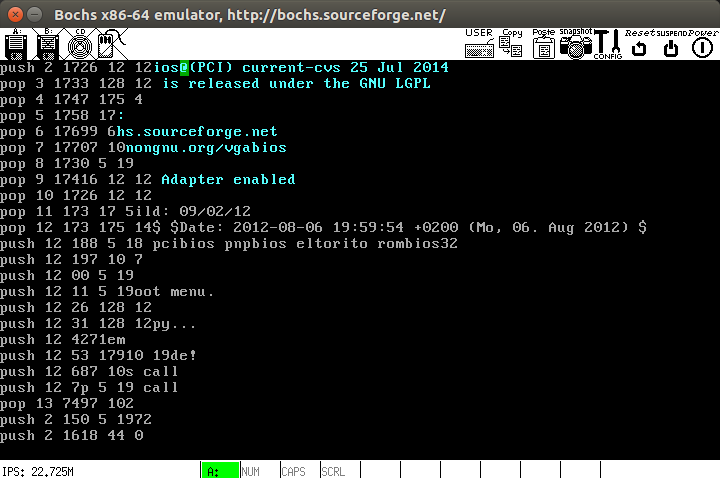
\includegraphics[scale=0.6]{assets/ex8finish.png}
    \caption{生产者消费者问题实验现象\label{fig:ex8finish}} 
    \end{center} 
\end{figure} 

\section{实验总结}
    \subsection{实验心得}
    本实验难度不大。在实验六和实验七都正常工作的前提下,完成本实验花费的时间
    较少。\\ 

    本实验在完成时依旧遇到了很严重的bug,见第\ref{sec:bug}节的讨论。\\ 

    由于一些历史遗留的原因,以往的实验中的系统调用都没有涉及参数的传递。但
    本实验中,内核的申请、释放信号量和P、V操作,都涉及到参数的传递。故本
    实验又再次修改了中断发生时的逻辑,在兼容以往实验的基础上,允许中断服务
    程序接收参数。本实验所有的操作都最终在系统调用中实现。用户的库函数仅仅
    只是一个封装,封装了中断的调用。如此即可将用户程序和内核代码解耦。确保
    用户程序无法直接修改和触碰到内核的变量。在以后开启特权级后,即可做到
    真正的保护功能。
    \subsection{BUG汇总}\label{sec:bug}
    \subsubsection{没有初始化}
    gcc有时会初始化全局变量,有时不会。在本实验中,我仅仅修改了部分``无关
    紧要''的代码后,发现全局变量没有被初始化了。这导致了全局变量被零初始化,
    最终导致不断抛出常规保护错误的异常。\\ 

    在一步一步跟踪到发生常规保护错误的代码后,我就发现了变量的值很意外得
    为零。于是我猜想初始话没有发生。我试着写一个init函数,在函数中显式得初始化
    全局变量,并在内核初始化时调用init函数。如此即解决了这个问题。
    \subsubsection{数组长度忘记声明}
    由于忘记声明了数组长度,我把数组的初始话写成了type arr[] = \{\}的形式。
    这导致了gcc实际上不在内存中为数组分配空间(分配的空间大小为0,数组长度为
    0)。\\ 

    由于一些巧合的原因,虽然数组没有被分配到空间,但其前8个元素的值都``恰好''没有被改写。只有第9个元素和以后的元素被
    覆盖了。于是导致了前8个系统调用都正常工作,但其后的系统调用都会产生常规保护异常。\\ 

    调试时的截图如图\ref{fig:error}所示。在右侧把内存中的值打印出来时,前面的值都是正确的。都与左侧的符号表中的值相符合。
    但是数组后面的值出错了。

    
    
    \begin{figure}[!hbt]
        \begin{center}
        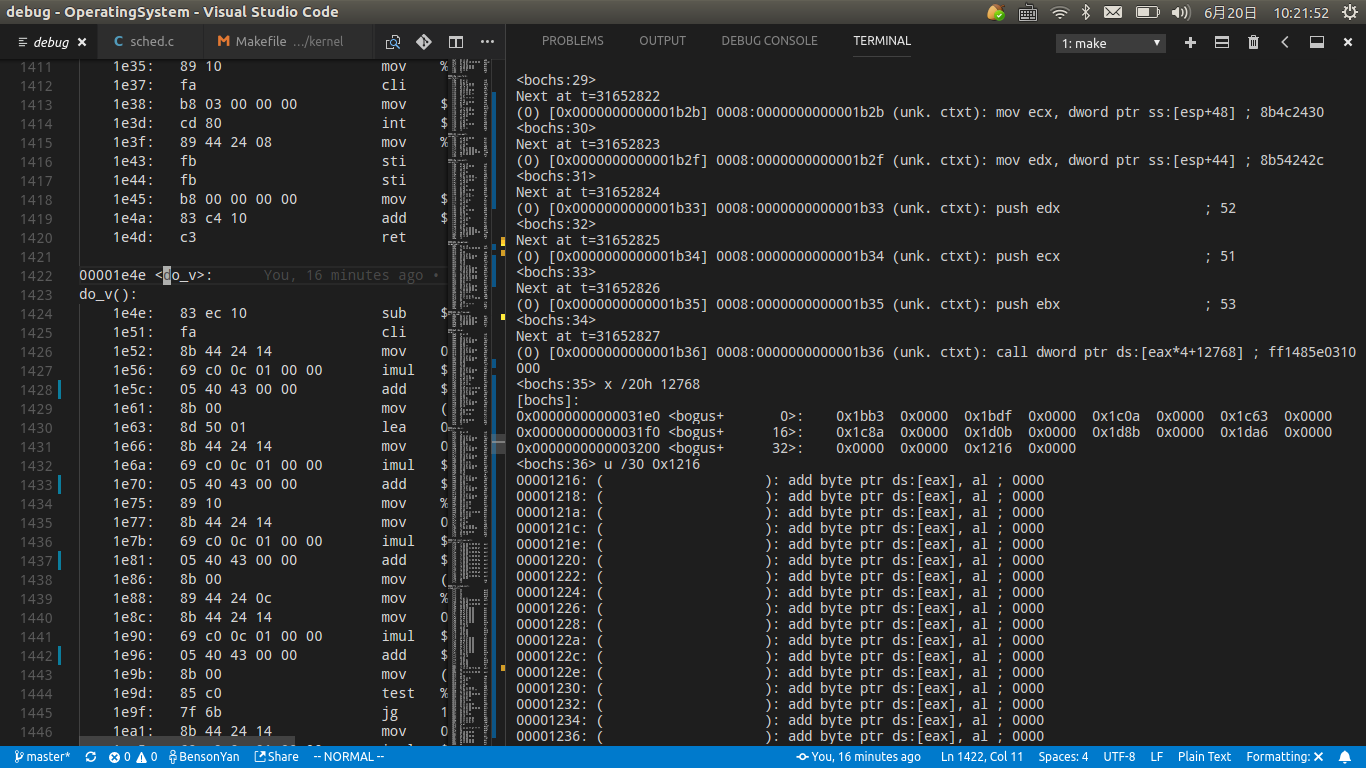
\includegraphics[scale=0.3]{assets/error.png}
        \caption{调试时数组的值出错的截图\label{fig:error}} 
        \end{center} 
    \end{figure} 
    
\begin{appendices}
\section{参考文献} \label{sec:reference}
\begin{enumerate}
    \item https://blog.csdn.net/longintchar/article/details/50602851 \\
    16位和32位汇编指令的不同(尤其是push指令)
    \item https://www.ibiblio.org/gferg/ldp/GCC-Inline-Assembly-HOWTO.html\#s1 \\
    GCC 内嵌汇编的书写。
  \end{enumerate}
\end{appendices}
\end{document}
